\documentclass[a4paper]{article}
\usepackage[utf8]{inputenc} %Кодировка
\usepackage[T2A]{fontenc}
\usepackage[english, russian]{babel}
\usepackage{amsmath, amsfonts, amssymb} %Мат пакеты
\usepackage{fancybox, fancyhdr}
\pagestyle{fancy}
\fancyhf{}
\usepackage{graphicx}
\fancyfoot[R]{\thepage} %Справа снизу подпись номера страницы
\fancyhead[L]{Физика. Билет №22. Моменты инерции простых однородных твёрдых тел. Теорема Гюйгенса-Штейнера}
\setcounter{page}{1} %счётчик нумерации страниц
\headsep=10mm %Отступ 
\usepackage{xcolor}
\usepackage{hyperref}

\begin{document}
	
	\section{Моменты инерции для простых однородных тел} 
	\begin{flushleft}
	Момент инерции ($I = \int_m r^2 dm$) - мера инертности во вращательном движении вокруг оси. Он характеризует сопротивление тела изменению его угловой скорости при приложении вращательного момента. \linebreak
	Момент инерции тела зависит от его массы и распределения массы относительно оси вращения.  \linebreak
\end{flushleft}
\subsection*{Вывод формулы}
\begin{flushleft}
	\begin{figure}[h]
		
		\centering
		
		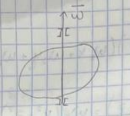
\includegraphics[width=0.8\linewidth]{images/22_1.png}
		
		\caption{Тело с осью вращения}
		
		\label{fig:mpr}
		
	\end{figure}
	$\omega_z : L_z$ \linebreak
	$\omega_z -$ угловая скорость\linebreak
	$L_z -$ момент импульса (нас интересует) \linebreak
	$L_z = I_{zx} \omega_x + I_{zy} \omega_y + I_{zz} \omega_z =  I_{zz} \omega_z$ \linebreak
	$ \vec{\omega} = \omega_z  \vec{k}$ \linebreak
	$(x^2 + y^2)$ - это расстояние до оси вращения \linebreak
	$I_{zz} = \int_m (x^2 + y ^ 2)dm = \int_m R^2 dm$
\end{flushleft}

	\subsection*{Примеры расчёта моментов инерции для тел симметричной формы:}
	\begin{flushleft}
		Тонкий стержень массы $m$ и длины $L$, если ось вращения перпендикулярна стержню и проходит через его центр масс: $I = \frac{mL^2}{12}$ 
		\linebreak \linebreak
		Тонкое кольцо массы $m$ и радиуса $R$, если ось вращения перпендикулярна плоскости кольца и проходит через центр масс: $I = mR^2$ (радиус постоянный, поэтому просто интегрируем).
		\linebreak \linebreak
		Тонкостенная труба (полый цилиндр) массы $m$, радиуса $R$ и длины $L$, если ось вращения совпадает с осью симметрии трубы: $I = mR^2$ (радиус постоянный, просто интегрируем).
		\linebreak \linebreak
		Сплошной цилиндр массы $m$ и радиуса $R$, если ось вращения совпадает с осью симметрии цилиндра: $I = \frac{mR^2}{2}$.
		\linebreak
		(Для вывода распишите: $dm = \frac{m}{\pi R^ 2}2\pi dr$)
		
	\end{flushleft}
	\section{Теорема Гюйгенса-Штейнера (теорема о переносе оси)}
	\begin{flushleft}
		Теорема позволяет рассчитать момент инерции тела относительно оси, параллельной оси, проходящей через центр масс, на расстоянии $a$ от неё. \linebreak \linebreak
		Формула: $I_B = I_A + ma^2$, где $I_B$ — момент инерции относительно новой оси, $I_A$ — момент инерции относительно оси, проходящей через центр масс, $m$ — масса тела, $a$ — расстояние между осями. \linebreak \linebreak
		Применение: если точка $A$ совпадает с центром масс тела, то $I_B = I_C + ma^2$, где $I_C$ — момент инерции относительно оси через центр масс. Момент инерции тела относительно оси, проходящей через его центр масс, является наименьшим для всех параллельных осей.
		
	\end{flushleft}
	\subsection*{Вывод}
	\begin{flushleft}
			\begin{figure}[h]
			
			\centering
			
			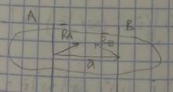
\includegraphics[width=0.8\linewidth]{images/22_2.png}
			
			\caption{основа вывода формулы}
			
			\label{fig:mpr}
			
		\end{figure}
		$J_A = \int_{контур} R_A ^ 2 dm$ \linebreak
		$J_B = \int_{контур} (\vec{R_A} - \vec{a}) ^ 2 dm = ... = I_A + ma^2 - 2 \vec{a}\vec{R_c}m$ \linebreak
		$R_c$ - расстояние до оси А
	\end{flushleft}
	\subsection*{Пример применения теоремы Гюйгенса-Штейнера}
	
	\textbf{Задача:} Рассчитать момент инерции тонкого стержня массы \( m \) и длины \( L \) относительно оси, проходящей через один из его концов и перпендикулярной стержню.
	
	\textbf{Решение:}
	
	1. \textbf{Момент инерции относительно центра масс (ось \( A \)):}
	\[
	I_A = \frac{m L^2}{12}
	\]
	
	2. \textbf{Расстояние между осями \( A \) и \( B \) (ось через конец стержня):}
	\[
	a = \frac{L}{2}
	\]
	
	3. \textbf{Применение теоремы Гюйгенса-Штейнера:}
	\[
	I_B = I_A + m a^2
	\]
	Подставляем значения:
	\[
	I_B = \frac{m L^2}{12} + m \left( \frac{L}{2} \right)^2
	\]
	\[
	I_B = \frac{m L^2}{3}
	\]
	
	\textbf{Ответ:} Момент инерции тонкого стержня относительно оси, проходящей через его конец, равен \( \frac{m L^2}{3} \).
	
\end{document}